\documentclass[tikz,border=2mm]{standalone}
\usetikzlibrary{calc,quotes,intersections, angles}
\usepackage{tkz-euclide} %for right angle marker

\begin{document}
    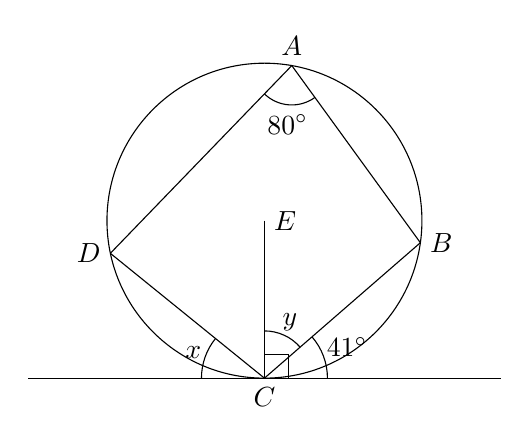
\begin{tikzpicture}[scale=2]
    % mark points on circle
        \coordinate[label = right:$E$] (E) at (0,0);
        \coordinate[label=below:$C$] (C) at (-90:1);
        \coordinate[label=above:$A$] (A) at (80:1);

    % draw chords and circle
        \draw[name path=circ] (0,0) circle (1);
        \draw (E) -- (C);
    %     \draw (B) -- (C);
    %     \draw (E) -- (C);
        

    % draw tangent
    \draw (C) -- ($(C)!1.5!-90:(E)$) coordinate (L);
    \draw (C) -- ($(C)!1.5!90:(E)$) coordinate (M);

    %
    \path[name path=CB] (C) -- ($(C)!1.5!-49:(E)$);
    \path[name path=CD] (C) -- ($(C)!1.5!51:(E)$);
    \path[name intersections={of=CB and circ, by={temp,B}}];
    \path[name intersections={of=CD and circ, by={D,temp}}];

    \draw (C) -- (B);
    \draw (C) -- (D);

    % Label points B and D
    \node at (B) [anchor=west] {$B$};
    \node at (D) [anchor= east] {$D$};

    \draw (A) -- (B);
    \draw (A) -- (D);
    
    \pic [draw, "$80^\circ$", angle eccentricity=1.5, angle radius = 0.5cm] {angle = D--A--B};
    \pic [draw, "$x$", angle eccentricity=1.2, angle radius = 0.8cm] {angle = D--C--M};
    \pic [draw, "$y$", angle eccentricity=1.3, angle radius = 0.6cm] {angle = B--C--E};
    \pic [draw, "$41^\circ$", angle eccentricity=1.4, angle radius = 0.8cm] {angle = L--C--B};

    %marking right angles
    \tkzMarkRightAngle[size=.15](L,C,E);
        
    \end{tikzpicture}
\end{document}